\chapter{Bandit-Based Model Selection}

In the previous chapters, we have been working with a single model and a single controller for any given task. When given a new task however, a new choice needs to be made for what model and controller is most suitable. Rather than assuming we have a single high-fidelity model of a deformable object interacting with its environment, our approach is to have multiple models available for use, any one of which may be useful at a given time. We do not assume these models are correct, we simply treat the models as having some measurable \textit{utility} to the task. The \textit{utility} of a given model is the expected reduction in task error when using this model to generate robot motion. As the task proceeds, the utility of a given model may change, making other models more suitable for the current part of the task. However, without testing a model's prediction, we do not know its true utility. Testing every model in the set is impractical, as all models would need to be tested at every step, and performing a test changes the state of the object and may drive it into a local minimum. The key question is then which model should be selected for testing at a given time.

The central contribution of this chapter is framing the model selection problem as a Multi-armed Bandit (MAB) problem where the goal is to find the model that has the highest utility for a given task. An arm represents a single model of the deformable object; to ``pull'' an arm is to use the arm's model to generate and execute a velocity command for the robot. The reward received is the reduction in task error after executing the command. In order to determine which model has the highest utility we need to explore the model space, however we also want to exploit the information we have gained by using models that we estimate to have high utility. One of the primary challenges in performing this exploration versus exploitation trade-off is that our models are inherently coupled and non-stationary; performing an action changes the state of the system which can change the utility of every model, as well as the reward of pulling each arm. While there is work that frames robust trajectory selection as a MAB problem~\cite{Koval2015}, we are not aware of any previous work which either 1) frames model selection for deformable objects as a MAB problem; or 2) addresses the coupling between arms for non-stationary MAB problems.

In our experiments, we show how to formulate a MAB problem with coupled arms for Jacobian-based models. We perform our experiments on three synthetic systems, and on three deformable object manipulation tasks in the Bullet Physics~\cite{Coumans2010} simulator. We demonstrate that formulating model selection as a MAB problem is able to successfully perform all three manipulation tasks. We also show that our proposed MAB algorithm outperforms previous MAB methods on synthetic trials, and performs competitively on the manipulation tasks.

%%%%%%%%%%%%%%%%%%%%%%%%%%%%%%%%%%%%%%%%%%%%%%%%%%%%%%%%%%%%%%%%%%%%%%%%%%%%%%%%%%%%%%%%%%%%%%%%%%%%%%%%%%%%%%%%%%%%%%%

\section{Problem Statement}

Using similar notation as previous chapters, let a \textit{deformation model} be defined as a function 
\begin{equation}
    \DeformForwardFn : \gripperVspace \rightarrow \deformCspace
\end{equation}
which maps a change in robot configuration $\grippervel$ to a change in object configuration $\deformvel$. Let $\modelset$ be a set of $\nmodels$ deformable models which satisfy this definition. Each model is associated with a robot command function
\begin{equation}
    \DeformBackwardFn : \deformCspace \times \reals^\ndeformpoints \rightarrow \gripperVspace
\end{equation}
which maps a desired deformable object velocity $\deformvel$ and weight $\Pinvweight$ (Section~\ref{sec:reducing_error}) to a robot velocity command $\grippervel$. $\DeformBackwardFn$ and $\DeformBackwardFn$ also take the object and robot configuration $(\deformconfig, \gripperconfig)$ and environment $\obstacle$ as additional input, however these are frequently omitted for brevity. When a model $\modelidx$ is selected for testing, the model generates a gripper command
\begin{equation}
    \grippervel_{\modelidx}(t) = \DeformBackwardFn_\modelidx(\deformvel(t), \Pinvweight(t))
    \label{eqn:grippervel}
\end{equation}
which is then executed for one unit of time, moving the deformable object to configuration $\deformconfig(t+1)$.

The problem we address in this chapter is which model $\modelidx \in \modelset$ to select in order to to move $\ngrippers$ grippers such that the points in $\deformconfig$ align as closely as possible with some task-defined set of $\ntargetpoints$ target points $\target \subset \reals^3$, while avoiding gripper collision and excessive stretching of the deformable object. Each task defines a function $\ErrorFn$ which measures the alignment error between $\deformconfig$ and $\target$. The method we present is a local method which picks a single model $\modelidx_{*}$ at each timestep to treat as the true model. This model is then used to reduce error as much as possible while avoiding collision and excessive stretching. 
\begin{equation}
    \modelidx^* = \argmin_{\modelidx \in \modelset} \ErrorFn(\target, \deformconfig(t+1))
    \label{eqn:modelselection}
\end{equation}
We show that this problem can be treated as an instance of the multi-arm non-stationary dependent bandit problem.

%%%%%%%%%%%%%%%%%%%%%%%%%%%%%%%%%%%%%%%%%%%%%%%%%%%%%%%%%%%%%%%%%%%%%%%%%%%%%%%%%%%%%%%%%%%%%%%%%%%%%%%%%%%%%%%%%%%%%%%

\section{Bandit-Based Model Selection}

The primary difficulty with solving~\eqref{eqn:modelselection} directly is that the effectiveness of a particular model in minimizing error is unknown. It may be the case that no model in the set produces the optimal option, however, this does not prevent a model from being useful. In particular the \textit{utility} of a model may change from one task to another, and from one configuration to another as the deformable object changes shape, and moves in and out of contact with the environment. We start by defining the utility $\utility_\modelidx(t) \in \reals$ of a model as the expected improvement in task error $\ErrorFn$ if model $\modelidx$ is used to generate a robot command at time $t$. If we know which model has the highest utility then we can solve~\eqref{eqn:modelselection}. This leads to a classic exploration versus exploitation trade-off where we need to explore the space of models in order to learn which one is the most useful, while also exploiting the knowledge we have already gained.  The multi-armed bandit framework is explicitly designed to handle this trade-off.

In the MAB framework, each arm represents a model in~$\modelset$; to pull arm $\modelidx$ is to command the grippers with velocity $\grippervel_\modelidx(t)$ (Eq.~\ref{eqn:grippervel}) for 1 unit of time. We then define the \textit{reward} $\reward_\modelidx(t+1)$ after taking action $\grippervel_\modelidx(t)$ as the improvement in error
\begin{equation}
    \reward_\modelidx(t+1) = \ErrorFn(t) - \ErrorFn(t+1) = \utility_\modelidx(t) + \utilityobsnoise
    \label{eqn:observedreward}
\end{equation}
where $\utilityobsnoise$ is a zero-mean noise term. The goal is to pick a sequence of arm pulls to minimize total expected regret $\totalregret(T_f)$ over some (possibly infinite) horizon $T_f$
\begin{equation}
    E[\totalregret(T_f)] = \sum_{t=1}^{T_f} (E[\reward^*(t)] - E[\reward(t)])
    \label{eqn:totalregret}
\end{equation}
where $\reward^*(t)$ is the reward of the best model at time $t$. The next section describes how to use bandit-based model selection for deformable object manipulation.

%%%%%%%%%%%%%%%%%%%%%%%%%%%%%%%%%%%%%%%%%%%%%%%%%%%%%%%%%%%%%%%%%%%%%%%%%%%%%%%%%%%%%%%%%%%%%%%%%%%%%%%%%%%%%%%%%%%%%%%

\section{Multi-Armed Bandit Formulation for Deformable Object Manipulation}

\todoin{Rename this section or the whole chapter}

\begin{algorithm}[ht]
    \caption{MainLoop$(\obstacle, \beta, \lambda)$}
    \begin{algorithmic}[1]
        \State $t \gets 0$
        \State $\RelaxedDistMatrix \gets$ GeodesicDistanceMatrix$(\deformconfig_{relaxed})$
        \State $\modelset \gets$ InitializeModels$(\RelaxedDistMatrix)$
        \State InitialzeBanditAlgorithm()
        \State $\deformconfig(0) \gets$ SensePoints()
        \State $\robotconfig(0) \gets$ SenseRobotConfig()
        \While{true}
            \State $\modelchosen \gets $ SelectArmUsingBanditAlgorithm()
            
            \State $\target \gets$ GetTargets()
            \State $\correspondences \gets$ CalculateCorrespondences$(\deformconfig_t, \target)$
            \State $\deformvel_e, \Pinvweight_e \gets$ FollowNavigationFunction$(\deformconfig_n, \correspondences)$
            \State $\deformvel_s, \Pinvweight_s \gets$ StretchingCorrection$(\RelaxedDistMatrix, \stretchmax, \deformconfig)$
            \State $\deformvel_d, \Pinvweight_d \gets$ CombineTerms$(\deformvel_e, \Pinvweight_e, \deformvel_s, \Pinvweight_s, \stretchweightfactor)$

            \State $\grippervel_d \gets \DeformBackwardFn_m(\deformvel_d, \Pinvweight_d)$
            \State $\grippervel \gets$ ObstacleRepulsion$(\grippervel_d, \obstacle, \obsavoidfactor)$
            
            \State CommandConfiguration$(\gripperconfig(t) + \grippervel)$

            \State $\deformconfig(t + 1) \gets$ SensePoints$()$
            \State $\robotconfig(t + 1) \gets$ SenseRobotConfig$()$
            \State UpdateBanditAlgorithm$()$
            
            \State $t \gets t + 1$
        \EndWhile
    \end{algorithmic}
    \label{alg:mab_mainloop}
\end{algorithm}

Our algorithm~(Alg.~\ref{alg:mab_mainloop}) can be broken down into four major sections and an initialization block. In the initialization block we pre-compute the geodesic distance (see Figure~\ref{fig:geodesic}) between every pair of points in $\deformconfig$ when the deformable object is in its ``natural'' or ``relaxed'' state and store the result in $\RelaxedDistMatrix$. These distances are used to construct the deformation models~(Section~\ref{sec:diminishing_rigidity}), as well as to avoid overstretching the object (Section~\ref{sec:stretching_correction}).
At each iteration we: 
\begin{enumerate}
    \item pick a model to use to achieve the desired direction~(Section~\ref{sec:bandit_algorithms}); 
    \item compute the task-defined desired direction to move the deformable object~(Section~\ref{sec:reducing_error}); 
    \item generate a velocity command using the chosen model~(Section~\ref{sec:stretching_avoidance_controller}); 
    \item modify the command to avoid obstacles~(Section~\ref{sec:stretching_avoidance_controller});
    \item update bandit algorithm parameters~(Section~\ref{sec:bandit_algorithms}).
\end{enumerate}

%%%%%%%%%%%%%%%%%%%%%%%%%%%%%%%%%%%%%%%%%%%%%%%%%%%%%%%%%%%%%%%%%%%%%%%%%%%%%%%%%%%%%%%%%%%%%%%%%%%%%%%%%%%%%%%%%%%%%%%

\section{Algorithms for MAB}
\label{sec:bandit_algorithms}

Previous solutions~\cite{Auer2002,Granmo2010} to minimizing~\eqref{eqn:totalregret} assume that rewards for each arm are normally and independently distributed and then estimate the mean and variance of each Gaussian distribution.  We test three algorithms in our experiments: Upper Confidence Bound for normally distributed bandits UCB1-Normal, Kalman Filter Based Solution to Non-Stationary Multi-arm Normal Bandits (KF-MANB), and our extension of KF-MANB, Kalman Filter Based Solution to Non-Stationary Multi-arm Normal Dependent Bandit (KF-MANDB).

\subsection{UCB1-Normal}
The UCB1-Normal algorithm~\cite{Auer2002} (Alg.~\ref{alg:ucb1normal}) treats each arm (model) as independent, estimating an optimistic Upper Confidence Bound (UCB) for the utility of each model. The model with the highest UCB is used to command the robot at each timestep. This algorithm assumes that the utility of each model is stationary, gradually shifting from exploration to exploitation as more information is gained. While our problem is non-stationary and dependant, we use UCB1-Normal as a baseline algorithm to compare against due to its prevalence in previous work.

\begin{algorithm}[t]
    \caption{UCB1-Normal - reproduced from~\cite{Auer2002}}
    \label{alg:ucb1normal}
    \begin{algorithmic}
        \For{$t = 1,2,\dots$}
            \vspace{-11pt}
            \State{
                \begin{itemize}
                    \item If there is an arm which has been pulled less than $\ceil*{8 \log t}$ times then pull this arm. If multiple arms qualify, we select the arm that has been pulled less, selecting the arm with the lower index in the case of a tie.
                    \item Otherwise pull arm $j$ that maximizes
                        \begin{equation*}
                            \bar \utility_j + \sqrt{16 \cdot \frac{q_j - n_j \bar \utility_j^2}{n_j - 1} \cdot \frac{\ln(t-1)}{n_j}}
                        \end{equation*}
                        where $\bar \utility_j$ is the average reward obtained from arm~$j$, $q_j$ is the sum of squared rewards obtained from arm~$j$, and $n_j$ is the number of times arm~$j$ has been pulled so far.
                    \item Update $\bar \utility_j$ and $q_j$ with the obtained reward $r_j$.
                \end{itemize}
            }
        \EndFor
    \end{algorithmic}
\end{algorithm}


\subsection{KF-MANB}
The Kalman Filter Based Solution to Non-Stationary Multi-arm Bandit (KF-MANB) algorithm~\cite{Granmo2010} (Alg.~\ref{alg:kf-manb}) uses independent Kalman filters to estimate the utility distribution of each model, and then uses Thompson sampling~\cite{Agrawal2012} to chose which model to use at each timestep. Because this algorithm explicitly allows for non-stationary reward distributions, it is able to ``switch'' between models much faster than UCB1-Normal.

\renewcommand{\algorithmicrequire}{\textbf{Input:}}
\renewcommand{\algorithmicensure}{\textbf{Initialization:}}
\begin{algorithm}[t]
    \caption{KF-MANB - reproduced from~\cite{Granmo2010}}
    \label{alg:kf-manb}
    \begin{algorithmic}
        \Require Number of bandit arms $\nmodels$; Observation noise $\observationnoisefactor^2$; Transition noise $\transitionnoisefactor^2 \utilityprocessscale^2$.
        \Ensure $\bar \utility_1(1) = \bar \utility_2(1) = \dots = \bar \utility_\nmodels(1) = A$; $\sigma_1(1) = \sigma_2(1) = \dots = \sigma_\nmodels(1) = B$; \textit{\# Typically, $A$ can be set to $0$, with $B$ being sufficiently large}
        \For{$t = 1,2,\dots$}
            \vspace{-11pt}
            \State{
                \begin{enumerate}
                    \item{For each arm $j \in \{1,\dots,\nmodels\}$}, draw a value $x_j$ randomly from the associated \textit{normal} distribution $f(x_j;\bar \utility_j(t),\sigma_j(t))$ with the parameters $(\bar \utility_j(t),\sigma_j(t))$.
                    \item{Pull the arm $i$ whose drawn $x_i$ is the largest one:
                        \begin{equation*}
                            i = \argmax_{j \in \{1,\dots,\nmodels\}} x_j.
                        \end{equation*}
                    }
                    \item{Receive reward $\tilde \reward_i$ from pulling arm $i$, and update parameters as follows:
                        \begin{itemize}
                            \item{Arm $i$:
                                \begin{align*}
                                    \bar \utility_i(t+1)      &= \frac{(\sigma_i^2(t) + \transitionnoisefactor^2 \utilityprocessscale^2) \cdot \tilde r_i + \observationnoisefactor^2 \cdot \bar \utility_i(t)}{\sigma_i^2(t) + \transitionnoisefactor^2 \utilityprocessscale^2 + \observationnoisefactor^2} \\
                                    \sigma_i^2(t+1) &= \frac{(\sigma_i^2(t) + \transitionnoisefactor^2 \utilityprocessscale^2) \observationnoisefactor^2}{\sigma_i^2(t) + \transitionnoisefactor^2 \utilityprocessscale^2 + \observationnoisefactor^2}
                                \end{align*}
                            }
                            \item{Arm $j \neq i$:
                                \begin{align*}
                                    \bar \utility_j(t+1)      &= \bar \utility_j(t) \\
                                    \sigma_j^2(t+1) &= \sigma^2_j(t) + \sigma_{tr}^2
                                \end{align*}
                            }
                        \end{itemize}
                    }
                \end{enumerate}}
        \EndFor
    \end{algorithmic}
\end{algorithm}


\subsection{KF-MANDB}
We also propose a variant of KF-MANB, replacing the independent Kalman filters with a single joint Kalman filter (Alg.~\ref{alg:kf-mandb}). This enables us to capture the correlations between models, allowing us to learn more from each pull. We start by defining utility as a linear system with Gaussian noise with process model $\utility(t+1) = \utility(t) + \utilityprocessnoise$ and observation model $\utilityobs(t) = C(t)\utility(t) + \utilityobsnoise$ where $\utility(t)$ is our current estimate of the relative utility of each model, while $\utilityprocessnoise$ and $\utilityobsnoise$ are zero-mean Gaussian noise terms. $C(t)$ is a row vector with a 1 in the column of the model we used and zeros elsewhere. The variance on $\utilityobsnoise$ is defined as $\observationnoisefactor^2 \utilityprocessscale^2$. $\utilityprocessscale$ is a tuning parameter to scale the covariance to match the reward scale of the specific task, while $\observationnoisefactor$ controls how much we believe each new observation.

\renewcommand{\algorithmicrequire}{\textbf{Input:}}
\renewcommand{\algorithmicensure}{\textbf{Initialization:}}
\begin{algorithm}[t]
    \caption{KF-MANDB}
    \label{alg:kf-mandb}
    \begin{algorithmic}
        \Require Number of bandit arms $\nmodels$; Observation noise $\observationnoisefactor^2$; Transition noise $\transitionnoisefactor^2 \utilityprocessscale^2$.
        \Ensure $\bar \utility(1) = A \in \reals^\nmodels$; $\utilityprocessnoisecovar(1) = B \in \reals^{\nmodels \times \nmodels}$; \textit{\# Typically, $A$ can be set to $0$, with $B \succ 0$} and sufficiently large
        \For{$t = 1,2,\dots$}
            \vspace{-11pt}
            \State{
                \begin{enumerate}
                    \item{For each arm $j \in \{1,\dots,\nmodels\}$, generate a gripper velocity command $\grippervel_j$.}
                    \item{Draw a value $x = \begin{bmatrix}x_1 & \dots & x_\nmodels \end{bmatrix}^T$ randomly from the joint \textit{normal} distribution $f(x;\bar \utility(t),\utilityprocessnoisecovar(t))$ with the parameters $(\bar \utility(t),\utilityprocessnoisecovar(t))$.}
                    \item{Pull the arm $i$ whose drawn $x_i$ is the largest one:
                        \begin{equation*}
                            i = \argmax_{j \in \{1,\dots,\nmodels\}} x_j.
                        \end{equation*}
                    }
                    \item{Receive reward $\tilde \utilityobs_i$ from pulling arm $i$, and perform a standard Kalman filter prediction and update step:
                        \begin{itemize}
                            \item{Compute \textit{a priori} covariance estimate and Kalman gain:
                                \begin{align*}
                                    \utilityprocessnoisecovar_{tr}   &\mbox{ is calculated using Eq.~\ref{eqn:processnoise}} \\
                                    \hat \utilityprocessnoisecovar   &= \utilityprocessnoisecovar(t) + \utilityprocessnoisecovar_{tr} \\
                                    S                                &= C(t) \hat \utilityprocessnoisecovar C(t)^T + \observationnoisefactor^2 \\
                                    K                                &= \hat \utilityprocessnoisecovar C(t)^T S^{-1}
                                \end{align*}
                            }
                            \item{Compute \textit{a posteriori} utility and covariance estimates:
                                \begin{align*}
                                    \bar \utility(t + 1)             &= \bar \utility(t) - K \left( C(t) \bar \utility(t) - \tilde \utilityobs_i \right) \\
                                    \utilityprocessnoisecovar(t + 1) &= \hat \utilityprocessnoisecovar - K C(t) \hat \utilityprocessnoisecovar
                                \end{align*}
                            }
                        \end{itemize}
                    }
                \end{enumerate}
            }
        \EndFor
    \end{algorithmic}
\end{algorithm}

To define the process noise $\utilityprocessnoise$ we want to leverage correlations between models; if two model commands are similar at the current time, the utility of these models is likely correlated. To measure the similarity between two models $i$ and $j$ we use the angle between their gripper velocity commands $\grippervel_{i}$ and $\grippervel_{j}$. This similarity is then used to directly construct a covariance matrix for each arm pull:
{\begin{equation}
\begin{split}
    \utilityprocessnoise            &\sim \normal{0}{\utilityprocessnoisecovar_{tr}}\\
    \utilityprocessnoisecovar_{tr}  & = \transitionnoisefactor^2 \utilityprocessscale^2 (\correlationfactor \utilityprocessnoisecovar_{sim} + \left(1 - \correlationfactor\right) \eye)\\
    \utilityprocessnoisecovar_{sim,i,j} & = \frac{\langle \grippervel_{i}, \grippervel_{j} \rangle}{\| \grippervel_{i} \| \| \grippervel_{j} \|} = \cos \theta_{i,j} \enspace.
\label{eqn:processnoise}
\end{split}
\end{equation}}
$\transitionnoisefactor$ is the standard Kalman Filter transition noise factor tuning parameter. $\correlationfactor \in [0,1]$ is the correlation strength factor; larger $\correlationfactor$ gives more weight to the arm correlation, while smaller $\correlationfactor$ gives lower weight. When $\correlationfactor$ is zero then KF-MANDB will have the same update rule as KF-MANB, thus we can view KF-MANDB as a generalizion of KF-MANB, allowing for correlation between arms.

After estimating the utility of each model and the noise parameters at the current timestep, these values are then passed into a Kalman filter which estimates a new joint distribution. The next step is the same as KF-MANB; we draw a sample from the resulting distribution, then use the model that yields the largest sample to generate the next robot command. In this way we automatically switch between exploration and exploitation as the system evolves; if we are uncertain of the utility of our models then we are more likely to choose different models from one timestep to the next. If we believe that we have accurate estimates of utility, then we are more likely to choose the model with the highest utility.

%%%%%%%%%%%%%%%%%%%%%%%%%%%%%%%%%%%%%%%%%%%%%%%%%%%%%%%%%%%%%%%%%%%%%%%%%%%%%%%%%%%%%%%%%%%%%%%%%%%%%%%%%%%%%%%%%%%%%%%

\section{Experiments and Results}

\begin{table}[t]
\centering
\caption{Controller parameters}
\label{tab:controller_param_table}
\begin{tabular}{lcccccc}
\hline\noalign{\smallskip}
                                                        &                       & \makecell{Synthetic\\Trials} 
                                                                                & \makecell{Rope\\Winding}
                                                                                & \makecell{Table\\Coverage}
                                                                                & \makecell{Two Stage\\Coverage} \\
\noalign{\smallskip}\hline\noalign{\smallskip}
\makecell[l]{$\tanse{3}$ inner\\product constant}      & $\rotvelweight$        &   - & 0.0025 & 0.0025 & 0.0025 \\
\noalign{\smallskip}
\makecell[l]{Servoing max\\gripper velocity}           & $\grippervelmaxservo$  & 0.1 &    0.2 &    0.2 &    0.2 \\
\noalign{\smallskip}
\makecell[l]{Obstacle avoidance\\max gripper velocity} & $\grippervelmaxobs$    &   - &    0.2 &    0.2 &    0.2 \\
\noalign{\smallskip}
\makecell[l]{Obstacle avoidance\\scale factor}         & $\obsavoidfactor$      &   - &    200 &   1000 &   1000 \\
\noalign{\smallskip}
\makecell[l]{Stretching correction\\scale factor}      & $\stretchweightfactor$ &   - &  0.005 &   0.03 &   0.03 \\
\hline
\end{tabular}
\end{table}
\begin{table}[t]
\centering
\caption{KF-MANB and KF-MANDB parameters}
\label{tab:param_table}
\begin{tabular}{lcccccc}
\hline\noalign{\smallskip}
                                                            &                               & \makecell{Synthetic\\Trials} 
                                                                                            & \makecell{Rope\\Winding}
                                                                                            & \makecell{Table\\Coverage}
                                                                                            & \makecell{Two Stage\\Coverage} \\
\noalign{\smallskip}\hline\noalign{\smallskip}
\makecell[l]{Correlation strength factor\\(KF-MANDB only)}  & $\correlationfactor$          &  0.9 &   0.9 &   0.9 &   0.9 \\
\noalign{\smallskip}
Transition noise factor                                     & $\transitionnoisefactor^2$    &    1 &   0.1 &   0.1 &   0.1 \\
\noalign{\smallskip}
Observation noise factor                                    & $\observationnoisefactor^2$   &    1 &  0.01 &  0.01 &  0.01 \\
\noalign{\smallskip}\hline
\end{tabular}
\end{table}

We test our method on three synthetic tests and three deformable object manipulation tasks in simulation. The synthetic tasks show that the principles we use to estimate the coupling between models are reasonable; while the simulated tasks show that our method is effective at performing deformable object manipulation tasks. Table~\ref{tab:controller_param_table} shows the parameters used by the Jacobian-based controller, while Table~\ref{tab:param_table} shows the parameters used by the the bandit algorithms for all experiments. We chose these parameters by comparing performance across noise factors $\observationnoisefactor^2$ and $\transitionnoisefactor^2$ from $\{0.01, 0.1, 1, 10\}$ and correlation strength factor $\correlationfactor$ from $\{0.1, 0.5, 0.9, 0.99\}$. While performance on individual experiments could be marginally improved by using different values, we found that $\observationnoisefactor^2=0.01$, $\transitionnoisefactor^2=0.1$, and $\correlationfactor=0.9$ resulted in robust performance for all of our manipulation tasks. $\utilityprocessscale$ is set dynamically and discussed in Section~\ref{sec:synthetic_trials}.




\subsection{Synthetic Tests}
\label{sec:synthetic_trials}


For the synthetic tests, we set up an underactuated system that is representative of manipulating a deformable object with configuration $y \in \reals^n$ and control input $\dot x \in \reals^m$ such that $m < n$ and $\dot y = J \dot x$. To construct the Jacobian of this system we start with $J = \begin{bmatrix}\eye_{m \times m} \\ \mathbf{0}_{(n-m) \times m} \end{bmatrix}$ and add uniform noise drawn from $[-0.1, 0.1]$ to each element of $J$. The system configuration starts at $\begin{bmatrix}10 & \dots & 10\end{bmatrix}^T$ with the target configuration set to the origin. Error is defined as $\ErrorFn(t) = \| y(t) \|$, and the desired direction to move the system at each timestep is $\dot y_d(t) = - y(t)$. These tasks have no obstacles or stretching, thus $\obsavoidfactor, \stretchweightfactor,$ and $\grippervelmaxobs$ are unused. Rather than setting the utility noise scale $\utilityprocessscale$ \textit{a priori}, we use an annealing filter
\begin{equation}
    \utilityprocessscale(t+1) = \max(10^{-10}, 0.9 \utilityprocessscale(t) + 0.1 |\reward(t+1)|) \enspace.
\end{equation}
This enables us to track the changing available reward as the system gets closer to the target.

To generate a model for the model set we start with the true Jacobian $J$ and add uniform noise drawn from $[-0.025, 0.025]$ to each element of $J$. For an individual trial, each bandit algorithm uses the same $J$ and the same model set. Each bandit algorithm receives the same random number stream during a trial, ensuring that a more favourable stream doesn't bias results. We ran one small test using a $3 \times 2$ Jacobian with 10 arms in order to yield results that are easily visualised. The second and third tests are representative of the scale of the simulation experiments, using the same number of models and similar sizes of Jacobian as are used in simulation. A single trial consists of 1000 pulls (1000 commanded actions); each test was performed 100 times to generate statistically significant results. Our results in Table~\ref{tab:synthetic_results} show that KF-MANDB clearly performs the best for all three tests.


\begin{table}[ht]
\centering
\caption{Synthetic trial results showing total regret with standard deviation in brackets for all bandit algorithms for 100 runs of each setup.}
\label{tab:synthetic_results}
\begin{tabular}{cccccc}
\hline\noalign{\smallskip}
\makecell{\# of\\Models} & \makecell{\# of rows\\in $J$}    & \makecell{\# of cols\\in $J$} & UCB1-Normal & KF-MANB     & KF-MANDB \\
\noalign{\smallskip}\hline\noalign{\smallskip}
10                      & 3                                 & 2                             & 4.41 [1.65] & 3.62 [1.73] & 2.99 [1.40] \\
60                      & 147                               & 6                             & 5.57 [1.37] & 4.89 [1.32] & 4.53 [1.42] \\
60                      & 6075                              & 12                            & 4.21 [0.64] & 3.30 [0.56] & 2.56 [0.54] \\
\hline
\end{tabular}
\end{table}


\subsection{Simulation Trials}

\begin{figure}[t]
    \centering
    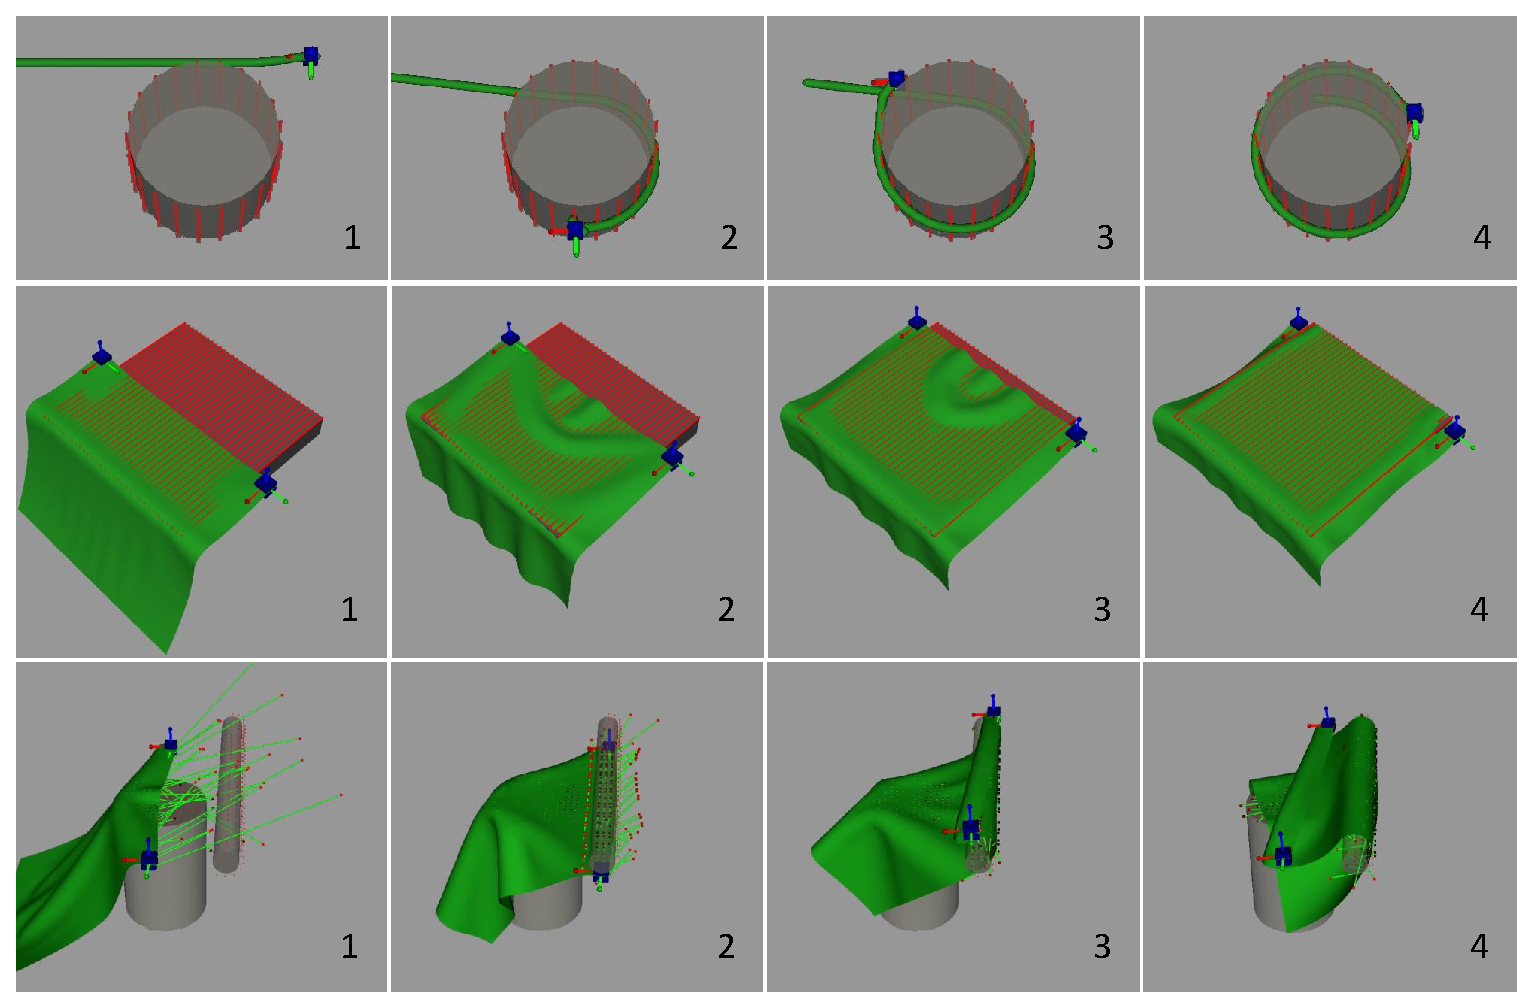
\includegraphics[width=\textwidth]{CombinedImages}
    \caption{Sequence of snapshots showing the execution of the simulated experiments using the KF-MANDB algorithm. The rope and cloth are shown in green, the grippers is shown in blue, and the target points are shown in red. The bottom row additionally shows $\deformvel_d$ as green rays with red tips.}
    \label{fig:simulation_task_screenshots}
\end{figure}

We now demonstrate the effectiveness of multi-arm bandit techniques on three example tasks, show how to encode those tasks for use in our framework, and discuss experimental results. The first task shows how our method can be applied to a rope, with the goal of winding the rope around a cylinder in the environment. The second and third tasks show the method applied to cloth. In the second task, two grippers manipulate the cloth so that it covers a table. In the third task, we perform a two-stage coverage task, covering portions of two different cylinders. In all three tasks, the alignment error $\ErrorFn(\deformconfig, \target)$ is measured as the sum of the distances between every point in $\target$ and the closest point in $\deformconfig$ in meters. Figure~\ref{fig:simulation_task_screenshots} shows the target points in red, and the deformable object in green. The video accompanying this paper shows the task executions.

All experiments were conducted in the open-source Bullet simulator~\cite{Coumans2010}, with additional wrapper code developed at UC Berkeley. The rope is modeled as a series of 49 small capsules linked together by springs and is 1.225m long. The cloth is modeled as a triangle mesh of size $0.5\text{m} \times 0.5\text{m}$ for the table coverage task, and size $0.5\text{m} \times 0.625\text{m}$ for the two-stage coverage task. We emphasize that our method does not have access to the model of the deformable object or the simulation parameters. The simulator is used as a ``black box'' for testing.\footnote{Our code is available at \url{https://github.com/UM-ARM-Lab/mab_ms}.}

In addition to the diminishing rigidity model introduced in Section~\ref{sec:diminishing_rigidity} we will also use \textit{adaptive Jacobian} models based on the work of \citet{Navarro-Alarcon2014}. This formulation uses an online estimation method to approximate $\Jacobian(\gripperconfig, \deformconfig)$.
First we with some estimate of the Jacobian $\tilde \Jacobian(0)$ at time $t = 0$ and then use the Broyden update rule~\cite{Broyden1965} to update $\tilde \Jacobian(t)$ at each timestep $t$
\begin{equation}
    \tilde \Jacobian(t) = \tilde J(t-1) + \ajrate \frac{\left( \deformvel(t) - \tilde \Jacobian(t-1) \grippervel(t) \right)}{\grippervel(t)^T \grippervel(t)} \grippervel(t)^T \enspace.
\end{equation}
This update rule depends on a update rate $\ajrate \in (0, 1]$ which controls how quickly the estimate shifts between timesteps.

We use models generated using the same parameters for all three tasks with a total of 60 models: 49 diminishing rigidity models with rotation and translational deformability values $\drktrans$ and $\drkrot$ ranging from 0 to 24 in steps of 4, as well as 11 adaptive Jacobian models with learning rates $\ajrate$ ranging from $1$ to $10^{-10}$ in multiples of 10. All adaptive Jacobian models are initialized with the same starting values; we use the diminishing rigidity Jacobian for this seed with $\drktrans=\drkrot=10$ for the rope experiment and $\drktrans=\drkrot=14$ for the cloth experiments to match the best model found in~\cite{Berenson2013}. We use the same strategy for setting $\utilityprocessscale$ as we use for the synthetic tests. 
%App~\ref{apx:param_table} shows all other parameters.

We evaluate results for the MAB algorithms as well as using each of the models in the set for the entire task. To calculate regret for each MAB algorithm, we create copies of the simulator at every timestep and simulate the gripper command, then measure the resulting reward $\reward_\modelidx(t)$ for each model. The reward of the best model $\reward^*(t)$ is then the maximum of individual rewards. As KF-MANB and KF-MANDB are not deterministic algorithms, each task is performed 10 times for these methods. All tests are run on an Intel Xeon E5-2683 v4 processor with 64 GB of RAM. UCB1-Normal and KF-MANB solve Eq.~\eqref{eqn:jacobianbackwardfunction_sim} once per timestep, while KF-MANDB solves it for every model in $\modelset$. Computation times for each test are shown in their respective sections.


\textit{Winding a Rope Around a Cylinder}: In the first example task, a single gripper holds a rope that is lying on a table. The task is to wind the rope around a cylinder which is also on the table (see Figure~\ref{fig:simulation_task_screenshots}). Our results~(Figure~\ref{fig:ropecylinder_results}) show that at the start of the task all the individual models perform nearly identically, starting to split at 2 seconds (when the gripper first approaches the cylinder) and again at 6 seconds. Despite our model set containing models that are unable to perform the task, our formulation is able to successfully perform the task using all three bandit algorithms. Interestingly, while KF-MANDB outperforms UCB1-Normal and KF-MANB in terms of regret, all three algorithms produce very similar results. Solving Eq.~\eqref{eqn:jacobianbackwardfunction_sim} at each iteration requires an average of 17.3~ms (std. dev. 5.5~ms) for a single model, and 239.5~ms (std. dev. 153.7~ms) for 60 models.

\begin{figure}[t]
    \centering
    \vspace{-0.1in}
    \subfloat{
        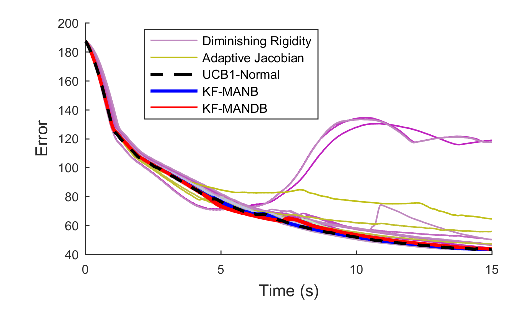
\includegraphics[width=0.45\textwidth]{rope_cylinder_wafr_tase_submission_error}
    }
    \subfloat{
        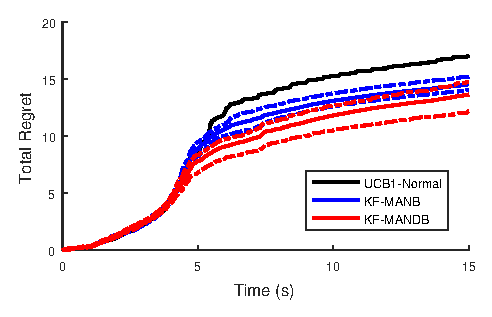
\includegraphics[width=0.45\textwidth]{rope_cylinder_wafr_tase_submission_total_regret}
    }
    \\
    \vspace{-0.15in}
    \subfloat{
        \hspace{-0.1in}
        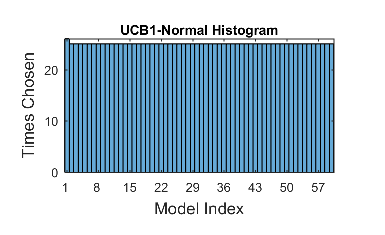
\includegraphics[width=0.35\textwidth]{rope_cylinder_wafr_tase_submission_UCB_histogram}
        \hspace{-0.25in}
    }
    \subfloat{
        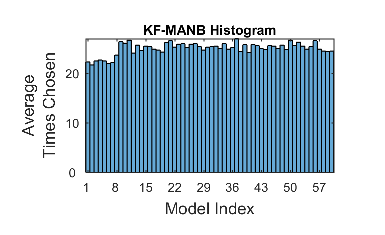
\includegraphics[width=0.35\textwidth]{rope_cylinder_wafr_tase_submission_KFMANB_histogram}
    }
    \subfloat{
        \hspace{-0.25in}
        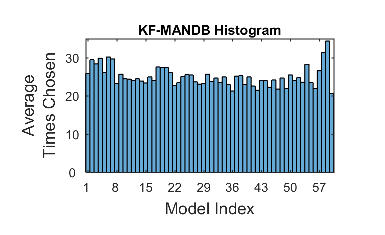
\includegraphics[width=0.35\textwidth]{rope_cylinder_wafr_tase_submission_KFMANDB_histogram}
        \hspace{-0.1in}
    }
    \vspace{-0.1in}
    \caption{Experimental results for the rope-winding task. Top left: alignment error for 10 trials for each MAB algorithm, and each model in the model set when used in isolation. UCB1-Normal, KF-MANB, KF-MANDB lines overlap in the figure for all trials. Top right: Total regret averaged across 10 trials for each MAB algorithm with the minimum and maximum drawn in dashed lines. Bottom row: histograms of the number of times each model was selected by each MAB algorithm; UCB1-Normal (bl), KF-MANB (bm), KF-MANDB (br).}
    \label{fig:ropecylinder_results}
\end{figure}



\textit{Spreading a Cloth Across a Table}: The second scenario we consider is spreading a cloth across a table. In this scenario two grippers hold the rectangular cloth at two corners and the task is to cover the top of the table with the cloth. All of the models are able to perform the task (see Figure~\ref{fig:clothtable_results}), however, many single-model runs are slower than the bandit methods at completing the task, showing the advantage of the bandit methods. When comparing between the bandit methods, both error and total regret indicate no performance difference between the methods. Solving Eq.~\eqref{eqn:jacobianbackwardfunction_sim} at each iteration requires an average of 89.5~ms (std. dev. 82.4~ms) for a single model, and 605.1~ms (std. dev. 514.3~ms) for 60 models.


\begin{figure}[t]
    \centering
    \vspace{-0.1in}
    \subfloat{
        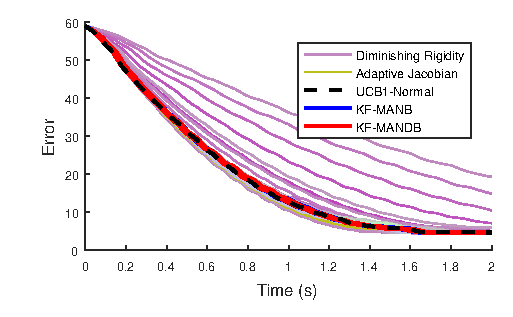
\includegraphics[width=0.45\textwidth]{cloth_table_wafr_tase_submission_error}
    }
    \subfloat{
        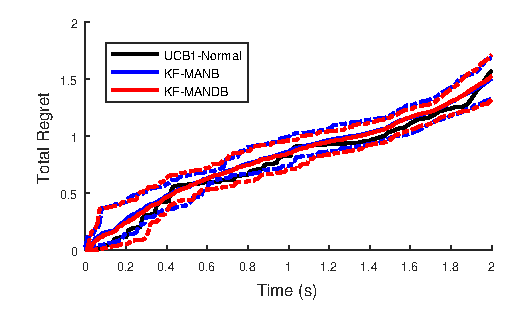
\includegraphics[width=0.45\textwidth]{cloth_table_wafr_tase_submission_total_regret}
    }
    \\
    \vspace{-0.15in}
    \subfloat{
        \hspace{-0.1in}
        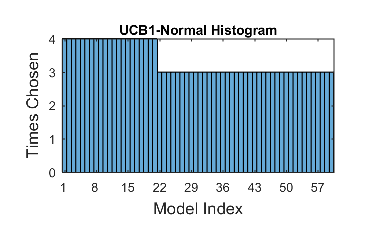
\includegraphics[width=0.35\textwidth]{cloth_table_wafr_tase_submission_UCB_histogram}
        \hspace{-0.25in}
    }
    \subfloat{
        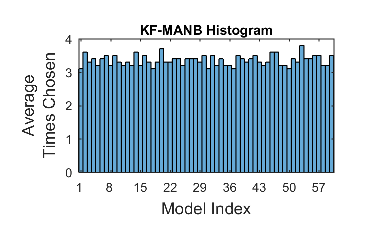
\includegraphics[width=0.35\textwidth]{cloth_table_wafr_tase_submission_KFMANB_histogram}
    }
    \subfloat{
        \hspace{-0.25in}
        \includegraphics[width=0.35\textwidth]{cloth_table_wafr_tase_submission_KFMANDB_histogram}
        \hspace{-0.1in}
    }
    \vspace{-0.1in}
    \caption{Experimental results for the table coverage task. See Figure~\ref{fig:ropecylinder_results} for description.}
    \label{fig:clothtable_results}
\end{figure}


\textit{Two-Part Coverage Task}: In this experiment, we consider a two-part task. The first part of the task is to cover the top of a cylinder similar to our second scenario. The second part of the task is to cover the far side of a second cylinder. For this task the \texttt{GetTargets} function used previously pulls the cloth directly into the second cylinder. The collision avoidance term then negates any motion in that direction causing the grippers to stop moving. To deal with this, we discretize the free space using a voxel grid, and then use Dijkstra's algorithm to find a collision free path between each cover point and every point in free space. We use the result from Dijkstra's algorithm to define a vector field that pulls the nearest (as defined by Dijkstra's) deformable object point $p_k$ along the shortest collision free path to the target point. This task is the most complex of the three (see Figure~\ref{fig:clothwafr_results}); many models are unable to perform the task at all, becoming stuck early in the task. We also observe that both KF-MANB and KF-MANDB show a preference for some models over others. Two interesting trials using KF-MANDB stand out; in the first the grippers end up on opposite sides of the second cylinder, in this configuration the physics engine has difficulty resolving the scene and allows the cloth to be pulled straight through the second cylinder. In the other trial the cloth is pulled off of the first cylinder, however KF-MANDB is able to recover, moving the cloth back onto the first cylinder. KF-MANDB and UCB1-Normal are able to perform the task significantly faster than KF-MANB, though all MAB methods complete the task using our formulation. Solving Eq.~\eqref{eqn:jacobianbackwardfunction_sim} at each iteration requires an average of 102.6~ms (std. dev. 30.6~ms) for a single model, and 565.5~ms (std. dev. 389.8~ms) for 60 models.

\begin{figure}[t]
    \centering
    \subfloat{
        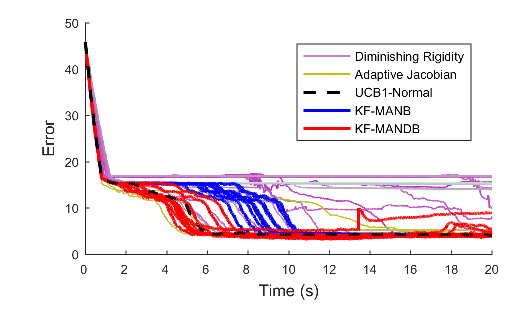
\includegraphics[width=0.45\textwidth]{cloth_wafr_wafr_tase_submission_error}
    }
    \subfloat{
        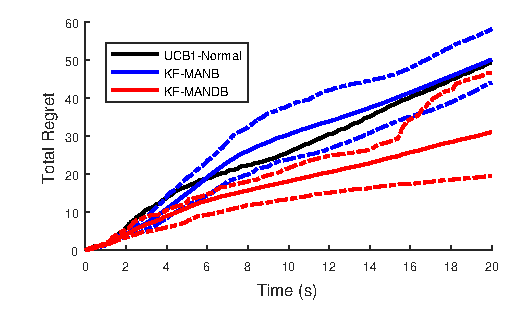
\includegraphics[width=0.45\textwidth]{cloth_wafr_wafr_tase_submission_total_regret}
    }
    \\
    \vspace{-0.15in}
    \subfloat{
        \hspace{-0.1in}
        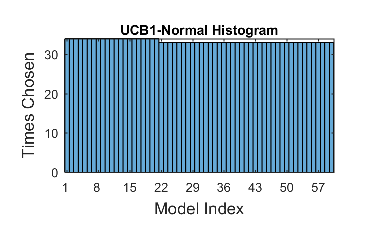
\includegraphics[width=0.35\textwidth]{cloth_wafr_wafr_tase_submission_UCB_histogram}
        \hspace{-0.25in}
    }
    \subfloat{
        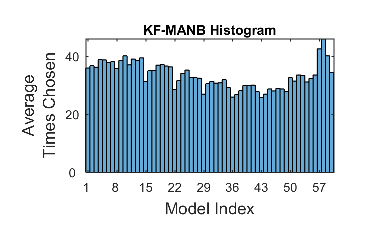
\includegraphics[width=0.35\textwidth]{cloth_wafr_wafr_tase_submission_KFMANB_histogram}
    }
    \subfloat{
        \hspace{-0.25in}
        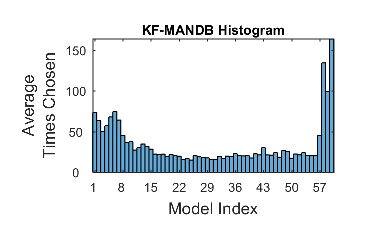
\includegraphics[width=0.35\textwidth]{cloth_wafr_wafr_tase_submission_KFMANDB_histogram}
        \hspace{-0.1in}
    }
    \vspace{-0.1in}
    \caption{Experimental results for the two-part coverage task. See Figure~\ref{fig:ropecylinder_results} for description.}
    \label{fig:clothwafr_results}
\end{figure}
